% make figure/table numbering nice
\setcounter{figure}{0}
\renewcommand{\thefigure}{S\arabic{figure}}
\renewcommand{\theHfigure}{S\thefigure}  % 

\newpage

% Gracefully skip missing SI image files during compilation
\let\origincludegraphics\includegraphics
\newcommand{\safeincludegraphics}[2][]{%
  \IfFileExists{#2}{\origincludegraphics[#1]{#2}}{\fbox{\parbox{0.9\linewidth}{\centering Missing figure file}}}%
}

% %%%%%%%%%%%%%%%%%%%%%%%%%%%%%%%%%%%%%%%
% ADD NEW SI ON TOP, WE COMMENT OUT/DELETE UNUSED LATER
%%%%%%%%%%%%%%%%%%%%%%%%%%%%%%%%%%%%%%%%%

\FloatBarrier

\begin{figure}
\begin{fullwidth}
\safeincludegraphics[width=\linewidth]{figures/rrr_peth_selectivity_comparison.pdf}
\caption{\textbf{Regional selectivity similarity and clustering along the cortical hierarchy: RRR (Posani et al.) versus PETH features.}
\textbf{a} RRR selectivity similarity \cite{posani2024rarely} uses each neuron's time-integrated absolute coefficient for every task variable as features; neurons are averaged within each region, features are standardized across regions, and cosine similarity is calculated between regional vectors.
\textbf{b} PETH selectivity similarity uses every PETH time bin as features; neurons are averaged within each region and cosine similarity is calculated between regional vectors. The horizontal axis uses the same Posani-style anatomical connectivity score as in \textbf{a}.
\textbf{c} Restricting to 67 regions with at least 50 UUID-matched neurons (10,477 included), regional DMN PETH geometry covaries with rank-5 RRR time-summed selectivity geometry.
\textbf{d} Rank-5 RRR silhouette $z$-score versus Posani hierarchy position \cite{harris2019hierarchical} for 24 regions passing RRR selectivity, neuron-count, and session-dominance criteria.
\textbf{e} Same analysis as \textbf{d}, but using the rank-3 ($\lambda=25$) RRR model selected automatically by three-fold cross-validation (mean CV $R^2$ 0.068 versus 0.066 for rank 5); neuron inclusion uses the rank-3 $\Delta R^2>0.015$, leaving 26 regions.
\textbf{f} PETH silhouette $z$-score versus the same hierarchy position for 34 regions passing the PETH neuron-count and session-dominance criteria.
\textbf{g} Across-region comparison of RRR mean absolute selectivity (Posani et al., Fig.~2c; authors' released coefficients) with BWM regional decoding scores \cite{international2025brain}, restricted to the task variables present in both analyses; RRR wheel selectivity is compared with both wheel-speed and wheel-velocity decoding. Each point is one of the 31 cortical regions with $\geq30$ RRR neurons and $\geq3$ regional decoding scores; both quantities are $z$-scored across these regions. Spearman $P$ values are uncorrected; after Bonferroni correction for five comparisons, feedback and wheel velocity remain significant (uncorrected $P<0.01$).
Dashed lines show the one-sided Bonferroni-corrected clustering criterion; its legend appears only in \textbf{d}. RRR has fewer regions than PETH because RRR first requires neuron-level prediction improvement over the null ($\Delta R^2>0.015$, evaluated for each rank); PETH uses all available cortical DMN neurons before both pipelines apply the $\geq50$-neuron and session-dominance criteria. Region-pair $P$ values use two-sided 10,000-permutation region-label QAP tests because pairs sharing regions are not independent.
\label{fig:rrr_peth_selectivity_comparison}
}
\end{fullwidth}
\end{figure}

\FloatBarrier

\begin{figure}
\centering
\safeincludegraphics[width=0.6\linewidth]{figures/movement_onset_subthreshold_wheel.pdf}
\caption{\textbf{Wheel motion before the reported movement onset does not predict choice.}
Data from 396 BWM sessions (128 mice, 11 laboratories).
\textbf{a} Example wheel traces (3 mice) aligned to the reported movement onset (\texttt{firstMovement\_times}) and sign-normalized to the eventual movement direction. Onset detection uses wheel displacement only, not choice or direction. The shaded 20~ms before onset was excluded from pre-onset measurements.
\textbf{b} Per-session percentage of trials in which the wheel direction matched the final choice, for net displacement from go cue to 20~ms before onset (blue) and for the first 50~ms after onset (green). Crosses show session median and interquartile range; the dashed line marks chance (50\%).
\label{fig:movement_onset_subthreshold_wheel}
}
\end{figure}


\FloatBarrier

\begin{figure}
\begin{fullwidth}
\safeincludegraphics[width=0.9\linewidth]{figures/umap_clustering_resolution.pdf}
\caption{\textbf{UMAP organization and cluster-mean response profiles across 
 k-means resolutions.} For each clustering resolution ($n_{\mathrm{clus}} = 10, 20, 30, 40, 100$), the top panel shows the mean trial-aligned response profile of each k-means cluster, and the bottom panel shows the corresponding 2D UMAP embedding of all neurons, colored by cluster identity. The cross-validated data was used here, i.e. the test half of the trials. This figure illustrates how embedding structure and average temporal response motifs evolve with increasing clustering granularity.}    
\label{fig:umap_clustering_resolution}
\end{fullwidth}
\end{figure}

\FloatBarrier


\begin{figure}
\begin{fullwidth}
\safeincludegraphics[width=\linewidth]{figures/rastermap_cross_validation.pdf}
\caption{\textbf{Split-trial cross-validation of rastermap.}
Trials are split into two sets (train and test) for each alignment and trial type, from which two concatenated feature vectors are computed for each cell. We apply rastermap algorithm on the training set, and apply the resulting ordering and cluster labels to both the train and test set. The majority of the patterns are preserved after cross-validation.
\label{fig:rastermap_cross_validation}
}
\end{fullwidth}
\end{figure}

\FloatBarrier


\begin{figure}
\begin{fullwidth}
\safeincludegraphics[width=\linewidth]{figures/rastermap_functional_categories.pdf}
\caption{\textbf{Functional cell clusters identified by rastermap and identification of some simple response categories.}
Left: Identification of some rastermap categories based on their response patterns: Stimulus response (orange; cluster 4), integrator (green; cluster 1-3, and 38), movement initiation (purple; cluster 10, 32, 34-37, 39, 41-42, and 61) and execution (red; cluster 72-75), sequences (blue; cluster 5-7, 11–20, 45–54, 56–59), feedback (pink; cluster 64-66, 78-82, 89, 94-95, and 97), and co-activation of feedback and movement (brown; cluster 0, 62-63, 67-68, 70-71, 76-77, 83-88, 90, and 96). 
Stimulus responders are classified as those with sharp early peaks when stimulus-algined, including during the visual stimulus onset and feedback period onset (e.g. for auditory responses). Stimulus integrator neurons are identified as active following the stimulus, with narrower activity packets when stimulus -aligned than movement aligned, with activity decay shortly before the movement period. Movement-related categories are identified based on a strong peak upon movement alignment relative to stimulus alignment. Different movement-related categories are based on the timing of response onset prior to movement, and on whether there is a continuation of activity into the movement period. 
Right: The corresponding neuron fraction of each group.
\label{fig:rastermap_categories}
}
\end{fullwidth}
\end{figure}


\FloatBarrier


\begin{figure}
\begin{fullwidth}
\safeincludegraphics[width=0.9\linewidth]{figures/sequence_shuffle_control.pdf}
\caption{\textbf{Additional shuffle control for sequence cells}
\textbf{a} We randomly shuffle the columns (time indices) of the sequence cells independently within each trial type, and re-sort the matrix with rastermap algorithm on the train set of trials (not shown) to apply the resulting ordering on the test set.
\textbf{b} Time-time correlation matrices of column-shuffled and re-sorted sequence neuron PETHs within each of the trial types, for the cross-validated test set of trials.
\textbf{c} Time-time autocorrelation across all stimulus-aligned trial types of the column-shuffled and re-sorted sequence cell activity.
\textbf{d} Overall pairwise Pearson correlation across all stimulus-aligned trial types for the stimulus/integrator neurons.
% 
\label{fig:sequence_shuffle_control}
}
\end{fullwidth}
\end{figure}

\FloatBarrier


\begin{figure}
\begin{fullwidth}
\safeincludegraphics[width=\linewidth]{figures/regional_cluster_composition_k25.pdf}
\caption{\textbf{Cluster composition per brain region}
Each panel shows the normalized fraction of neurons belonging to each of the 25 k-means clusters for a given Beryl brain region. Only regions with at least 50 neurons are shown (155 regions total). Colors correspond to k-means cluster identity. X-axis: cluster index (0–24); Y-axis: fraction of neurons in that cluster. All regions contain neurons from all clusters.
\label{fig:regional_cluster_composition}
}

\end{fullwidth}
\end{figure}

\FloatBarrier



\begin{figure}
\begin{fullwidth}
\safeincludegraphics[width=0.9\linewidth]{figures/specialization_metric_comparison.pdf}
\caption{\textbf{Specialization metrics compared} 
\textbf{a} Correlation between anatomical hierarchy (based on tract tracing \cite{harris2019hierarchical}) and specialization score based on k-means cluster counts is not significant.
\textbf{b} The correlation between the k-means and decoding-based specialization scores (Fig.~\ref{fig:anatomy_function}j) is stable under k-means cluster number variation after a minimal number of about 15 and is also significant when using the clusters provided by rastermap (green, red). Rastermap and k-means results converge as the number of clusters increases. 
\textbf{c} As with the k-means based specialization score in \textbf{a}, there is no correlation between decoding-based specialization and anatomical hierarchy score.
}    
\label{fig:specialization_metrics}
\end{fullwidth}
\end{figure}


\FloatBarrier


\begin{figure}
\begin{fullwidth}
\safeincludegraphics[width=\linewidth]{figures/prototype_vectors_k100.pdf}
\caption{\textbf{Average feature vectors for 100 k-means clusters, sorted hierarchically}
\textbf{a} The vectors are shown in order as used in Fig \ref{fig:mixed_selectivity}a when hierarchically sorting the coefficients of these 100 "basis" vectors (using Pearson correlation as the similarity metric), used to reconstruct the full response data. \textbf{b} In the same order, Pearson correlation matrix of coefficients across neurons, as in Fig \ref{fig:mixed_selectivity}b. 
\label{fig:prototype_vectors}
}
\end{fullwidth}
\end{figure}



\FloatBarrier


\begin{figure}
\begin{fullwidth}
\safeincludegraphics[width=\linewidth]{figures/mixed_selectivity_k40.pdf}
\caption{\textbf{Mixed selectivity analysis for 40 k-means clusters}
Same figure as Fig \ref{fig:mixed_selectivity} but with 40 k-means clusters as a basis (instead of 100 used in the main figure). Neurons are sorted as in Fig \ref{fig:mixed_selectivity}: real neurons by their k-means cluster (25 clusters, as in Fig.~\ref{fig:functional_response_structure}a), synthetic neurons by the nearest of the same 25 cluster centroids.
\label{fig:mixed_selectivity_k40}
}
\end{fullwidth}
\end{figure}

\FloatBarrier


\section{Dynamically evolving phase-specific functional similarity networks}

We have seen that distinct computations unfold in different task phases and involve partially separate neuron groups. A natural question is how different parts of the brain coordinate during these distinct phases. The field of fMRI, with a longer history of brain-wide recordings, has approached this question by performing multi-region functional graph analyses to identify functional subnetworks. The IBL dataset enables similar analyses, but at much higher ($\sim 10^3 \times$ or $\sim 1$ ms versus $\sim 1$ s) temporal and spatial ($\sim 10^3 \times$, with $\sim 60K$ cellular measurements in the supersession versus $\sim 60$ voxels) resolution. We now seek an area-wise analysis of dynamical functional similarity networks, or how the brain forms subnetworks to compute over different phases of the task, at high precision. 

To assay functional network-level interactions, we defined a functional similarity score between (Beryl) regions per task phase as a proxy for the strength between them, focusing on the following conditions: the resting period ("rest"); the enforced quiescent period ("quies") and pre-stimulus prior representation in this period ("$\mathrm{L_b}$" and "$\mathrm{R_b}$"); the stimulus response period in congruent trials (where the stimulus side equals the block side, i.e. "$\mathrm{L_{s}L_{c}L_{b}, s}$", "$\mathrm{R_{s}R_{c}R_{b}, s}$"); the stimulus response period in surprise trials (when the stimulus side is opposite the block side, i.e. "$\mathrm{L_{s}L_{c}R_{b}, s}$", "$\mathrm{R_{s}R_{c}L_{b}, s}$"); the stimulus response period in mistake trials ("mistake, s"); during movement initialization ('m'); in the movement period ("$\mathrm{L_{move}}$" and "$\mathrm{R_{move}}$"); and during feedback after correct ("feedbk1") and wrong ("feedbk0") trials. For each task phase, we subset the z-scored cellular feature vectors (as in Fig.~\ref{fig:architecture_task}f) to the relevant PETH time bins and trial conditions, construct region-wise smoothed 2D activity maps from those phase-specific cellular responses, and compute cosine similarity between the resulting region maps (see the following Method section and Fig.~\ref{fig:functional_networks}a), which yielded a similarity matrix across regions per task phase. All analyses use z-scoring normalization applied before subsetting to reduce baseline firing-rate differences and focus the comparison on response-pattern similarity. Thus similarity matrices compare regions within the same task phase using a common framework, ensuring comparability across phases. We then applied Louvain community detection to the similarity matrices to identify functional networks (region clusters with similar responses), and sorted neurons to be adjacent if they were assigned to the same community, Fig. ~\ref{fig:functional_networks}b-h (bottom-left in each panel). Note that the derived networks reflect phase-specific similarity of regional response motifs, not functional connectivity or direct inter-regional coupling. To assess which of the identified networks were reliable and meaningful, we applied three types of control analyses (see the following Methods section), as follows. Only networks that are deemed significant by the intersection of the three controls below are numbered in Fig.~\ref{fig:functional_networks}b-h. 

First, we identified which networks had a high 'network stability' score through split-trial comparisons (Fig. \ref{fig:network_stability}). We repeated Louvain clustering across several trial splits; for each identified cluster (community) in each split, we defined a binary regional participation vector (whether the region was in the community), and used these to create a regional membership similarity matrix across all clusters and all splits for a condition. We assigned a network stability score ($\in [0,1]$) defined by the average value of its regional membership similarity score (Table \ref{tab:cluster_stability}), and only communities with a stability score exceeding a threshold were deemed statistically stable. 

Second, to verify that the resulting networks identified as stable are different than would be obtained by random chance, we shuffled the region labels of all cells before computing the region-wise functional similarity scores and Louvain clustering. 
The resulting groupings were visually much more numerous and smaller than in the unshuffled data (Fig. \ref{fig:network_stability}), and their stability scores were well below the stability score threshold (Table \ref{tab:shuffled_cluster_stability}).

Our third control was based on the statistical significance of the functional responses of the identified networks relative to shuffles. We computed each network's PETH as a weighted (by region participation scores) average of the PETHs of the member regions, Fig. ~\ref{fig:functional_networks}b-e (line plots), and compared these to PETHs generated by randomly sampling the same number of regions from all recorded Beryl regions in the brain (gray lines in the line plots are the shuffled controls). A network was deemed significant in its functional properties if its PETH was significantly different from the random network PETHs for the majority of time bins ($\geq60\%$). 

We find that within each condition, brain states typically form a few non-orthogonal but distinct and regionally distributed similarity subnetworks, suggesting distinct processing modes, Fig.~\ref{fig:functional_networks}b-e. The regional composition of identified subnetworks varies substantially from one task phase and condition to the next, meaning that functional groupings are transient and rapidly shift across time and condition in the task, Fig.~\ref{fig:functional_networks}b-e (Swanson maps, right panels; darker colors indicate higher participation score). 
% For instance, the quiescence period exhibits of a multiplicity of small, decoupled, marginally significant subnetworks, with the sole significant network being predominantly subcortical (hindbrain), Fig.~\ref{fig:functional_networks}c. 
For the full concatenated PETHs ("concat", Fig.~\ref{fig:functional_networks}b), the three dominant subnetworks consist of neocortex-hippocampus, striatum-hypothalamus-midbrain–hindbrain, and cerebellum networks, and while in the congruent stimulus phase (Fig.~\ref{fig:functional_networks}c), the networks collapse to a dominant one, integrating the striatum-hypothalamus-midbrain-hindbrain network with some hippocampal and somato-sensory regions.
% This suggests that during surprise, the hippocampus becomes engaged with subcortical processing, consistent with \cite{brandman2020default, frank2022experiencing}. 
Movement initiation and movement, adjacent task phases, involve quite different subnetworks, reflecting dynamic reconfiguration (Fig.~\ref{fig:functional_networks}d): the movement initiation period exhibits three distinct subnetworks, one primarily neocortical engaging early sensory processing, somatosensory, and prefrontal areas, but also interacting with lateral hypothalamus, inferior colliculus, and cerebellum; the second is predominantly hippocampal-thalamic-dorsal striatum (CP) with somatosensory-secondary motor cortex engaged with midbrain and hindbrain; and the third is predominantly cerebellar with engagement of superior colliculus. Brain states in the movement period collapse into two statistically robust subnetworks, one (network 2) largely similar to the first movement initiation subnetwork (network 0), and the other a mixture of hippocampus, high-level association areas (RSP), midbrain (PAG), and hypothalamus. Finally, the incorrect feedback phase shows one subnetwork (Fig.~\ref{fig:functional_networks}e) that is similar to the motor-init network 2, presumably reflecting movement-related computations leaking through from the movement phase immediately earlier. 
% In what remains, there is significant but not perfect similarity between the subnetworks 2 in both feedback conditions; these exhibit high brainstem-cerebellar-striatal activation and possibly show common aspects of feedback processing. Subnetwork 1 in the correct feedback phase is distinct, involving cortico-cerebellar activation with widespread neocortical activity across low and high level cortical areas. 

One consistent pattern is that the within-condition subnetworks in every condition recapitulate the green-pink or cortical-subcortical response divide that we saw earlier at the single-cell level. This is evident in the graphs of Fig.~\ref{fig:functional_networks}, as well as when we form a similarity matrix of the region membership of subnetworks from all the task conditions, Fig.~\ref{fig:functional_networks}f. The subnetwork regional similarity matrix has a two-block structure, each with a representative subnetwork from most trial conditions. The upper block corresponds to primarily cortical processing networks, and the lower one to primarily subcortical processing networks. This cortical-subcortical separation is also supported by previous tract-tracing connectomics studies in the mouse brain, showing dense intra-cortical communities are largely segregated from dominant subcortical (thalamic, striatal, hypothalamic, brainstem) communities, with specific hub regions bridging the two compartments (\cite{Oh2014mesoscale, Ruminov2015wiring}). Finally, we compare these functional brain networks to established fMRI-based networks from the mouse brain (including default mode \cite{whitesell2021regional, fmri_Grandjean2017, fmri_Grandjean2020, fmri_Zerbi2015, fmri_Vafaii2024}, limbic/hippocampal \cite{fmri_Gutierrez-Barragan2022, fmri_Sforazzini2014, fmri_Grandjean2020, fmri_Bukhari2017}, salience \cite{fmri_Tsurugizawa2020, fmri_Grandjean2020, fmri_Vafaii2024}, sensorimotor \cite{fmri_Sforazzini2014, hike2025high, fmri_Zerbi2015, fmri_Grandjean2020}, and associated cortical networks \cite{fmri_Grandjean2017, fmri_Vafaii2024, fmri_Grandjean2020, fmri_Zerbi2015}; see Table~\ref{tab:fmri_networks} for datasets included) to determine whether there is a correspondence, Fig.~\ref{fig:functional_networks}g. The mouse fMRI sensory mode network (smn, Fig.~\ref{fig:functional_networks}g, last row) reassuringly overlaps with a subnetwork from the congruent stimulus conditions, but also with the more-cortical subnetworks from each of the movement initiation and movement conditions. However, beyond this similarity, we report few meaningful relationships between fMRI-defined subnetworks and our high spatio-temporal resolution brain networks. One would expect the resting or quiescent state network would correspond to the fMRI default mode networks (Fig.~\ref{fig:functional_networks}g, bottom row); however none of the quiescent / resting networks are reliable enough to survive the significance tests. The difference of recording conditions (resting state fMRI vs IBL task), the quantified dominance of subcortical processing in the brain throughout the course of the IBL task, the sparsity of fMRI maps in the mapping to Beryl regions even for cortical structures, and the lack of deep subcortical (e.g. midbrain, hindbrain, cerebellum) inclusion in the fMRI network studies are the likely causes of the discrepancy. We also note that our analyses do not measure trial-by-trial or moment-by-moment correlated fluctuations and therefore cannot establish functional connectivity or inter-regional coupling. The observed 'reconfiguration' refers to changes in functional similarity structure across task phases, not direct evidence for changing inter-regional communication.

Together, these results show in a spatiotemporally precise and brain-wide way that all brain areas participate in all functions, and that the brain forms emergent collective dynamical coalitions that rapidly reconfigure between task phases to enable accurate perceptual decision-making.

% \FloatBarrier

\begin{figure}
%\begin{fullwidth}
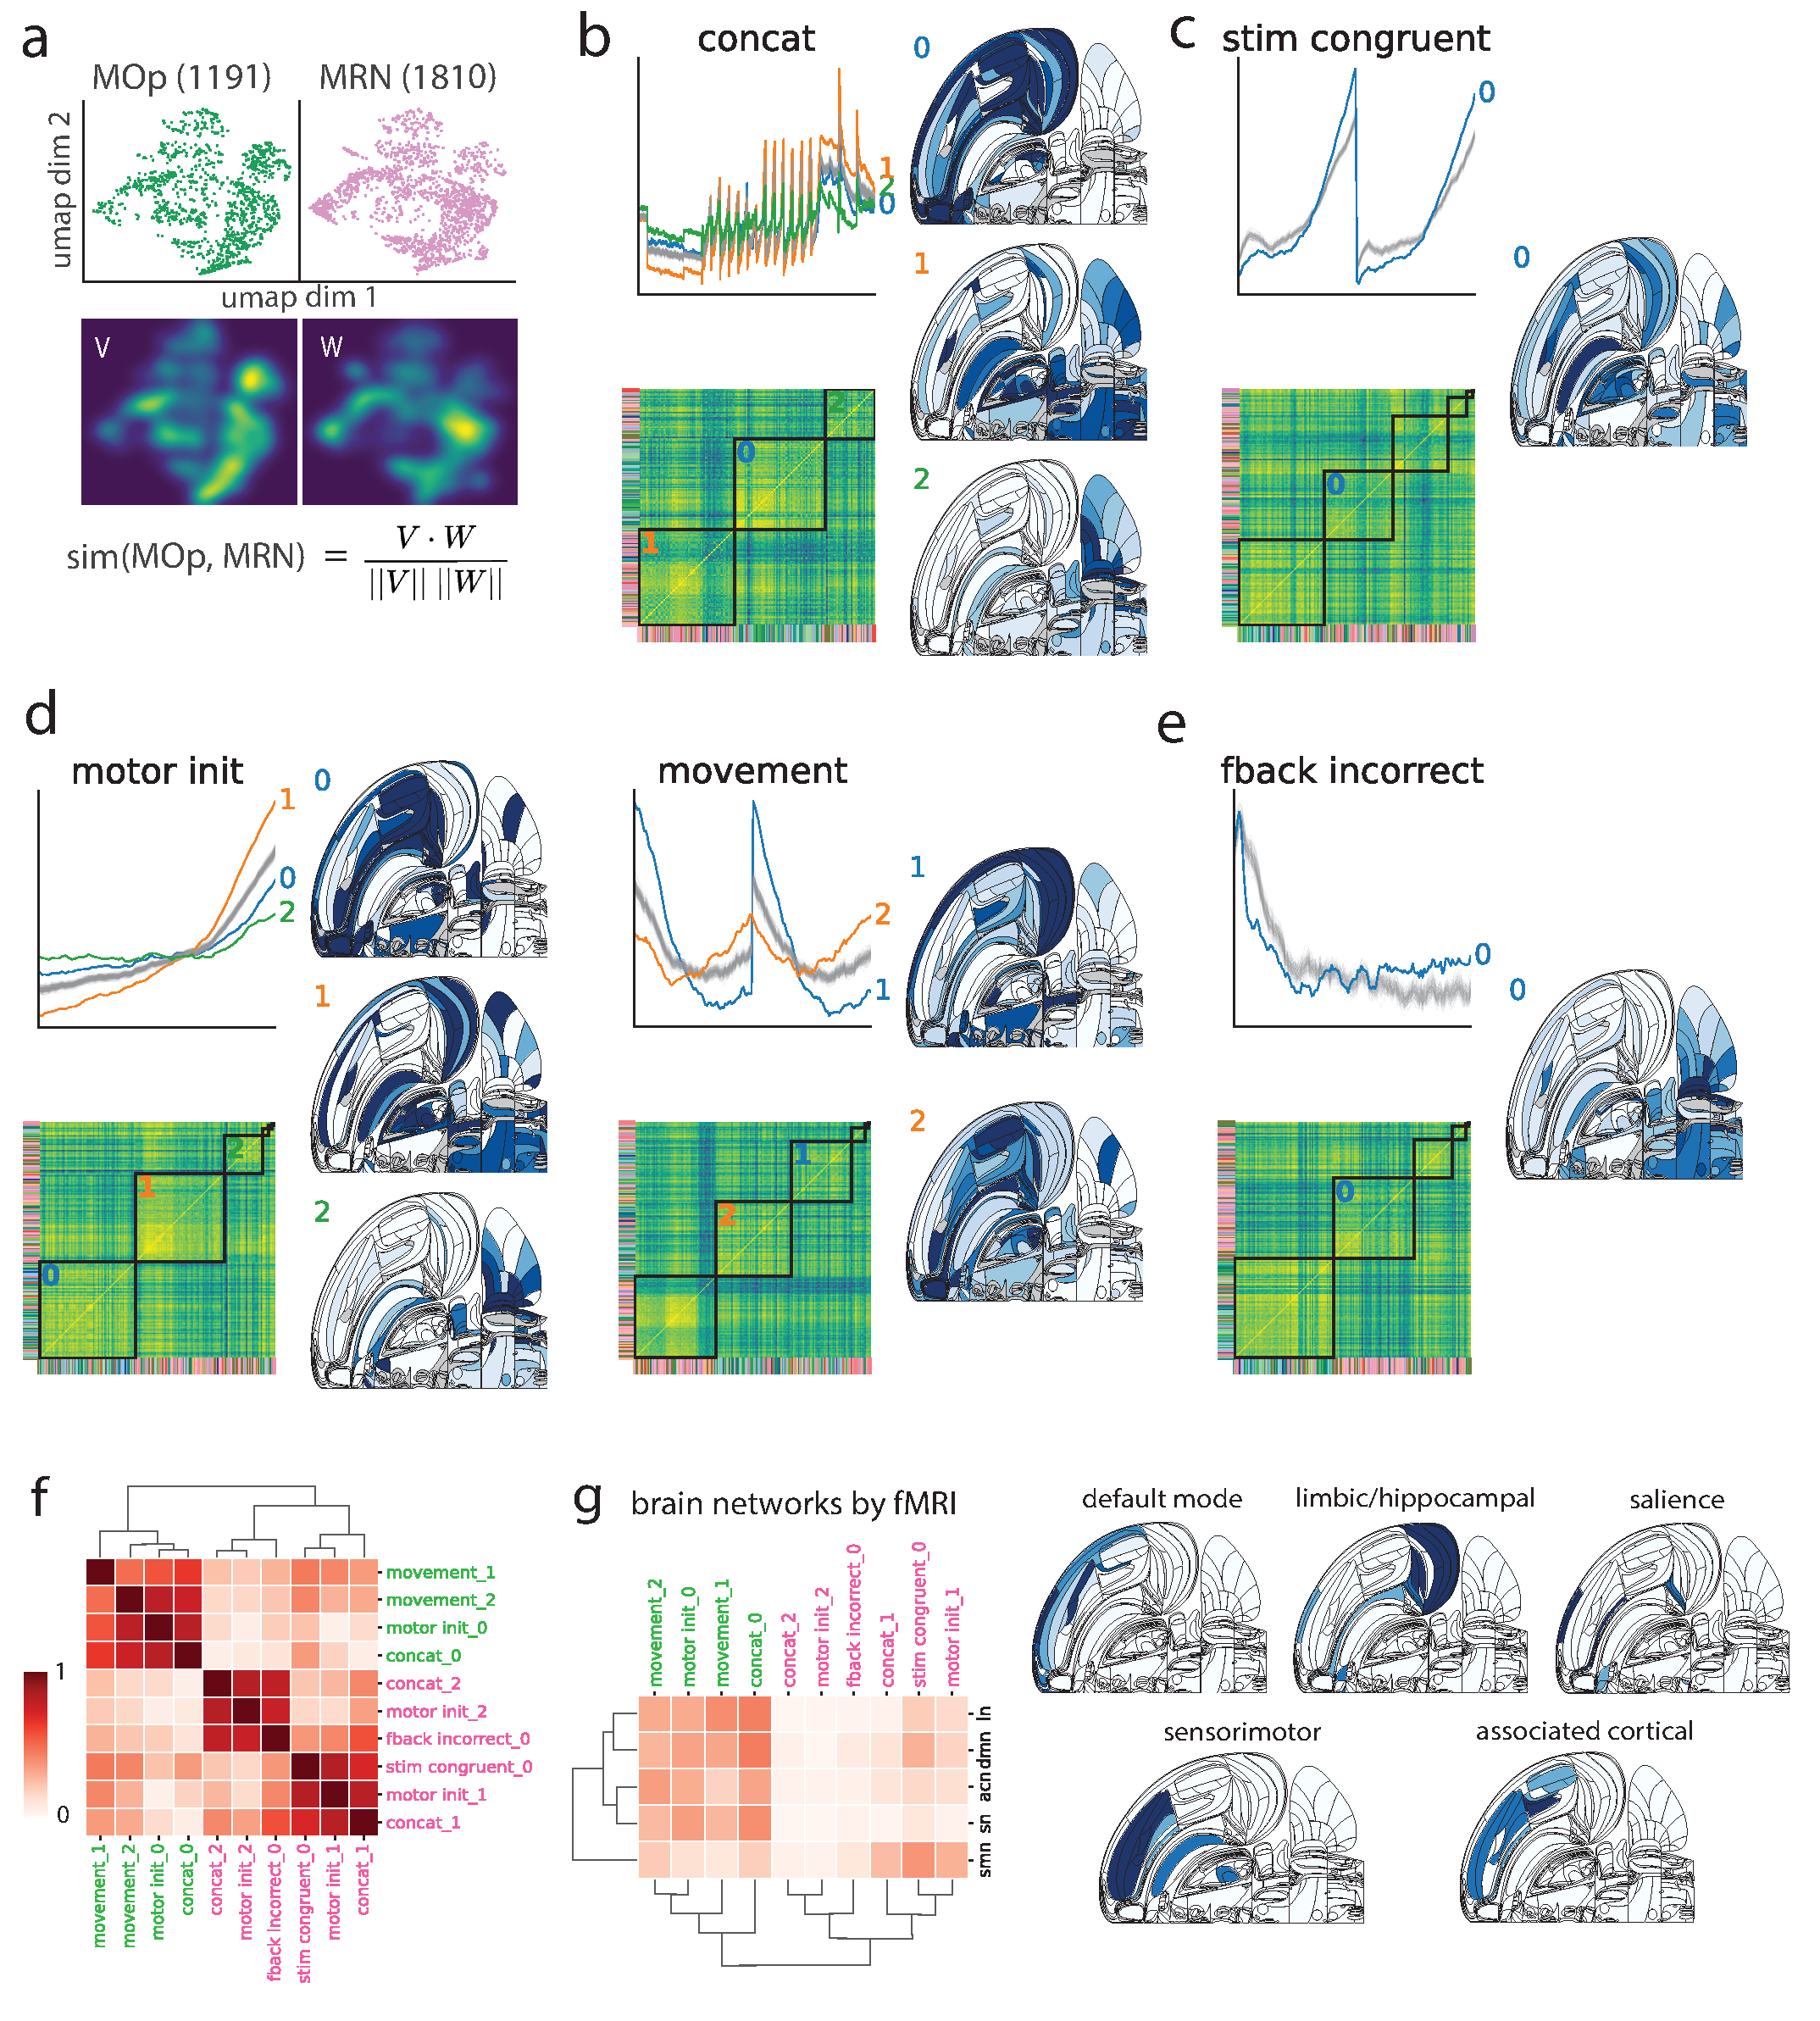
\includegraphics[width=0.8\linewidth]{figures/phase_specific_functional_networks.pdf}
\caption{ \textbf{Dynamically reconfiguring networks across different phases of the task.} \textbf{a} To compare functional responses between pairs of regions, we calculate a cosine similarity score of two regions’ cellular responses from a smoothed 2D embedding for the relevant task phase (here, shown for the concat condition which includes all task phases). \textbf{b-e} The regional similarity matrices are ordered by the Louvain community detection algorithm to identify groups of brain regions (networks) for various subsets of PETHs (task phases) shown in panels (b) through (e). The algorithm consistently shows a cortical-subcortical separation in two (or three) major networks across phases of the task, as evident in the Swanson maps (some clusters mostly subcortical, and the others mostly cortical + hippocampus) which show regional membership in these clusters (darker color indicates stronger membership from split-trial cross-validation). We also show line plots of the average PETHs for each network as compared to shuffled controls (gray), and the networks are only included in the current figure if they pass all three rounds of control analyses as described in the Methods. \textbf{f} Summary table showing cosine
similarity of Swanson maps between pairs of our defined networks, having two clear groups that correspond to the cortical-subcortical separation. \textbf{g} Cosine similarity of Swanson maps between our defined networks and canonical fMRI networks in the mouse brain (Swanson maps shown on the right), showing low similarity throughout. We combined multiple studies (see Table \ref{tab:fmri_networks} for details) for each mouse fMRI network, mapped the results of these studies onto Beryl regions, and colors in the Swanson maps indicate how consistently we find the regions being identified in a network, with darker color being more consistent.}
\label{fig:functional_networks}
%\end{fullwidth}
\end{figure}
% \FloatBarrier



\begin{table}[htbp]
\centering
\caption{Mapping of Functional Networks to Selected Literature, Mouse Sample Sizes, and Experimental States}
\label{tab:fmri_networks}
\small
\begin{tabularx}{\textwidth}{l l l X}
\toprule
\textbf{Network Domain} & \textbf{Citations} & \textbf{Sample Size ($N$)} & \textbf{Experimental Condition / State} \\
\midrule
\textbf{Default Mode} 
  & \cite{whitesell2021regional} & $N = 18$ & Anesthetized (isoflurane + medetomidine), resting-state \\
  & \cite{fmri_Grandjean2020} & $N = 610$ & Varied (awake and diverse anesthesia protocols across 14 sites) \\
  & \cite{fmri_Zerbi2015} & $N = 20$ & Anesthetized (medetomidine), resting-state \\
  & \cite{fmri_Grandjean2017} & $N = 45$ & Anesthetized (isoflurane + medetomidine), resting-state \\
  & \cite{fmri_Vafaii2024} & $N = 19$ & Anesthetized (isoflurane + pancuronium bromide), resting-state \\
\midrule
\textbf{Limbic / Hippocampal} 
  & \cite{fmri_Gutierrez-Barragan2022} & $N = 15$ / $15$ & Awake vs.\ Anesthetized (halothane), resting-state \\
  & \cite{fmri_Sforazzini2014} & $N = 15$ & Anesthetized (halothane), resting-state \\
  & \cite{fmri_Grandjean2020} & $N = 610$ & Varied (awake and diverse anesthesia protocols across 14 sites) \\
  & \cite{fmri_Bukhari2017} & $N = 50$ & Anesthetized (5 groups: isoflurane, propofol, medetomidine, combinations) \\
\midrule
\textbf{Salience} 
  & \cite{fmri_Tsurugizawa2020} & $N = 34$ & Awake, resting-state \\
  & \cite{fmri_Grandjean2020} & $N = 610$ & Varied (awake and diverse anesthesia protocols across 14 sites) \\
  & \cite{fmri_Vafaii2024} & $N = 19$ & Anesthetized (isoflurane + pancuronium bromide), resting-state \\
\midrule
\textbf{Sensorimotor} 
  & \cite{hike2025high} & $N = 9$ & Awake, resting-state \\
  & \cite{fmri_Sforazzini2014} & $N = 15$ & Anesthetized (halothane), resting-state \\
  & \cite{fmri_Zerbi2015} & $N = 20$ & Anesthetized (medetomidine), resting-state \\
  & \cite{fmri_Grandjean2020} & $N = 610$ & Varied (awake and diverse anesthesia protocols across 14 sites) \\
\midrule
\textbf{Associated Cortical / Laterocortical} 
  & \cite{fmri_Zerbi2015} & $N = 20$ & Anesthetized (medetomidine), resting-state \\
  & \cite{fmri_Grandjean2017} & $N = 45$ & Anesthetized (isoflurane + medetomidine), resting-state \\
  & \cite{fmri_Grandjean2020} & $N = 610$ & Varied (awake and diverse anesthesia protocols across 14 sites) \\
  & \cite{fmri_Vafaii2024} & $N = 19$ & Anesthetized (isoflurane + pancuronium bromide), resting-state \\
\bottomrule
\end{tabularx}
\end{table}



\subsection{Method: functional distance metric for brain region pairs}

We measure the functional distance between brain regions as follows. For a given region, the 2D umap embedding of all cells in this region (across recordings) is rasterized into a 256 x 256 pixel grid, with the cell density per pixel, then smoothed by applying a 2D Gaussian kernel with standard deviation of 10 pixels in each dimension and normalized such that the maximum grayscale per pixel is set to 1 and the minimum to zero. Given two such images for two regions, the images are flattened into vectors $\mathbf{v_1}, \mathbf{v_2}$ and the cosine similarity of the two vectors is defined as the functional distance between regions:

\[d_{1,2} = \frac{\mathbf{v_1} \mathbf{v_2}}{|\mathbf{v_1}| |\mathbf{v_2}|} \]


\subsection{Method: Louvain clustering}
We use \verb|sknetwork.clustering.Louvain| implemented in python to identify regional networks in the functional similarity matrices of different trial phases. We use the following parameters in the presented analysis: \verb|resolution=1.01, random_state=0|, after sweeping through parameters and other clustering algorithms that result in less reproducible networks with lower adjusted random index (\verb|sklearn.metrics.adjusted_rand_score|) and adjusted mutual information (\verb|sklearn.metrics.adjusted_mutual_info_score|). 

\subsection{Method: statistical significance of networks}
To assess which of the identified networks were reliable and meaningful, we applied three types of control analyses. 

First, we identified which networks had a high 'network stability' score through split-trial comparisons, as follows. We split all trials of a given type into two groups to obtain two independent feature vectors for each cell. Within each split, we re-computed similarity matrices and Louvain clusters (communities). We repeated this process four times to generate a total of eight sets of leave-half-out communities for each condition (each cross-validation set based on a random subset of $1/2$ the total trials). We compared region participation across the eight sets of communities to define a network stability score, as follows: All of the communities (for a given condition) in all the eight splits were assigned binary region participation vectors (of length equaling the number of Beryl regions), with $1$ indicating a region's membership in the community and $0$ otherwise, and we used these to create a regional membership similarity matrix across all clusters in all splits for the condition (Fig. \ref{fig:network_stability}), sorting the matrix elements by similarity to display the communities (SI Fig. \ref{fig:network_stability}, column 1). We only look at communities with sizes $>6$ when sorting the similarity matrix, meaning these communities are identified in at least 6 out of the 8 leave-half-out trial splits analysis. The network stability score of each community is defined as the average value (of the regional membership similarity score) within the community (Table \ref{tab:cluster_stability}): conceptually, if the same areas always appear together in one community across splits, the stability score would be 1; otherwise, it would take some value in the interval $[0,1]$. Communities with a stability score $<0.57$ (the average stability score across communities and across trial phases) were deemed statistically unstable and not numbered or plotted as Swanson maps in the main or supplemental figures. 

Second, to verify that the resulting stable identified networks are different than would be obtained by random chance, we shuffled the region labels of all cells before computing the region-wise functional similarity scores and Louvain clustering. 
The resulting groupings were visually much more numerous and smaller than in the unshuffled data (Fig.~\ref{fig:network_stability}). We quantitatively compared the shuffled data networks with the identified networks by computing the stability scores for the shuffled data networks. Most of the shuffled networks have grouping size stability scores below the criteria of stability score $>0.57$, and when comparing them across cross-validation splits, none of them show communities of size $\geq 6$(Table \ref{tab:shuffled_cluster_stability}).

Our third control was based on the statistical significance of the functional responses of the identified networks. The goal is to ensure the networks are a result of distinct and related responses of brain regions within a community rather than community-independent regional response variations. For each community, we computed its cluster PETH by a weighted average of the PETHs of the member regions (weighted by the participation scores of the regions, as defined in the next section in Methods), Fig. ~\ref{fig:functional_networks}b-e (line plot in each panel). We compared the community PETH with $1000$ control PETHs generated by randomly sampling the same number of regions as in the community from across the set of all recorded Beryl regions in the brain, and computing their average PETHs weighted by the same set of regional participation scores (randomly assigned to the random set of regions), Fig~\ref{fig:network_stability}. At each time bin, two p-values are defined by the fraction of times the shuffled controls are larger or smaller than the true PETH, and the true PETH is significantly different from the controls if either of the p-values are smaller than $0.01$. A community was deemed significant only if the resulting network PETHs were significantly different from the shuffled controls for the majority of the analysis time window.

Only networks that are deemed significant by the intersection of the three conditions above are numbered in Fig.~\ref{fig:functional_networks} of the main text. In Swanson maps, we show the membership of regions in each significant network, weighted by a network participation score. 

\subsection{Method: regional participation score of networks}
We define a region's participation score within a given network as the fraction of times the region is identified within the network across the eight-fold split-trial controls. If a region is identified in a given network in all eight splits, its participation score in the network is $1$, and if identified in none, its score is $0$.
For each network that passed the statistical significance tests, we show the Swanson maps of them in the results (Fig.\ref{fig:functional_networks}) by coloring the regions with the regional participation score. 

For each of the mouse fMRI networks, we combined results from multiple studies as shown in Table \ref{tab:fmri_networks}, mapped their included areas onto Beryl regions, and calculated the regional participation score across the studies we included. We show the Swanson maps of each network colored by the regional participation scores in Fig.\ref{fig:functional_networks}g.


\begin{table}[ht]
\centering
\renewcommand{\arraystretch}{1.2}
\begin{minipage}{0.48\textwidth}
\begin{tabular}{c|c|c}
\hline
\textbf{Cluster} & \textbf{Size} & \textbf{Stability} \\ \hline
\textcolor{red}{concat cluster 0} & \textcolor{red}{8} & \textcolor{red}{0.866} \\ \hline
\textcolor{red}{concat cluster 1} & \textcolor{red}{8} & \textcolor{red}{0.705} \\ \hline
\textcolor{red}{concat cluster 2} & \textcolor{red}{7} & \textcolor{red}{0.678} \\ \hline
concat cluster 3 & \textcolor{gray}{11} & \textcolor{gray}{0.107} \\ \hline
resting cluster 0 & \textcolor{gray}{2} & \textcolor{gray}{0.453} \\ \hline
resting cluster 1 & \textcolor{gray}{2} & \textcolor{gray}{0.39} \\ \hline
resting cluster 2 & \textcolor{gray}{2} & \textcolor{gray}{0.383} \\ \hline
resting cluster 3 & \textcolor{gray}{2} & \textcolor{gray}{0.333} \\ \hline
\textcolor{red}{quiescence cluster 0} & \textcolor{red}{7} & \textcolor{red}{0.65} \\ \hline
\textcolor{red}{pre-stim prior cluster 0} & \textcolor{red}{8} & \textcolor{red}{0.91} \\ \hline
\textcolor{red}{pre-stim prior cluster 1} & \textcolor{red}{8} & \textcolor{red}{0.886} \\ \hline
\textcolor{red}{mistake cluster 0} & \textcolor{red}{8} & \textcolor{red}{0.785} \\ \hline
\textcolor{red}{mistake cluster 1} & \textcolor{red}{8} & \textcolor{red}{0.624} \\ \hline
\textcolor{red}{mistake cluster 2} & \textcolor{red}{8} & \textcolor{red}{0.69} \\ \hline
mistake cluster 3 & \textcolor{gray}{8} & \textcolor{gray}{0.134} \\ \hline
\textcolor{red}{stim surprise cluster 0} & \textcolor{red}{6} & \textcolor{red}{0.721} \\ \hline
stim surprise cluster 1 & \textcolor{gray}{4} & \textcolor{gray}{0.638} \\ \hline
stim surprise cluster 2 & \textcolor{gray}{3} & \textcolor{gray}{0.7} \\ \hline
stim surprise cluster 3 & \textcolor{gray}{2} & \textcolor{gray}{0.592} \\ \hline
\textcolor{red}{stim congruent cluster 0} & \textcolor{red}{6} & \textcolor{red}{0.788} \\ \hline
\end{tabular}
\end{minipage}
\hfill
\begin{minipage}{0.48\textwidth}
\begin{tabular}{c|c|c}
\hline
\textbf{Cluster} & \textbf{Size} & \textbf{Stability} \\ \hline
stim congruent cluster 1 & \textcolor{gray}{9} & \textcolor{gray}{0.482} \\ \hline
stim congruent cluster 2 & \textcolor{gray}{8} & \textcolor{gray}{0.528} \\ \hline
stim congruent cluster 3 & \textcolor{gray}{18} & \textcolor{gray}{0.088} \\ \hline
\textcolor{red}{motor init cluster 0} & \textcolor{red}{8} & \textcolor{red}{0.899} \\ \hline
\textcolor{red}{motor init cluster 1} & \textcolor{red}{8} & \textcolor{red}{0.836} \\ \hline
\textcolor{red}{motor init cluster 2} & \textcolor{red}{8} & \textcolor{red}{0.759} \\ \hline
motor init cluster 3 & \textcolor{gray}{12} & \textcolor{gray}{0.153} \\ \hline
\textcolor{red}{movement cluster 0} & \textcolor{red}{7} & \textcolor{red}{0.839} \\ \hline
\textcolor{red}{movement cluster 1} & \textcolor{red}{6} & \textcolor{red}{0.729} \\ \hline
\textcolor{red}{movement cluster 2} & \textcolor{red}{8} & \textcolor{red}{0.661} \\ \hline
movement cluster 3 & \textcolor{gray}{15} & \textcolor{gray}{0.083} \\ \hline
fback correct cluster 0 & \textcolor{gray}{8} & \textcolor{gray}{0.564} \\ \hline
fback correct cluster 1 & \textcolor{gray}{8} & \textcolor{gray}{0.516} \\ \hline
fback correct cluster 2 & \textcolor{gray}{7} & \textcolor{gray}{0.523} \\ \hline
fback correct cluster 3 & \textcolor{gray}{7} & \textcolor{gray}{0.509} \\ \hline
fback correct cluster 4 & \textcolor{gray}{10} & \textcolor{gray}{0.057} \\ \hline
\textcolor{red}{fback incorrect cluster 0} & \textcolor{red}{8} & \textcolor{red}{0.617} \\ \hline
\textcolor{red}{fback incorrect cluster 1} & \textcolor{red}{8} & \textcolor{red}{0.602} \\ \hline
fback incorrect cluster 2 & \textcolor{gray}{22} & \textcolor{gray}{0.03} \\ \hline
fback incorrect cluster 3 & \textcolor{gray}{8} & \textcolor{gray}{0.353} \\ \hline
fback incorrect cluster 4 & \textcolor{gray}{5} & \textcolor{gray}{0.398} \\ \hline
\end{tabular}
\end{minipage}
\caption{\textbf{Stability scores for regional clusters}. Stability scores identified from comparing clusters that are identified from different trial splits for all trial phases. Size indicates the number of times a community is identified in the 8 leave-half-out trial splits analysis. Clusters with stability scores $>0.57$ and size $\geq6$ (marked as red) pass the stability criteria.}
\label{tab:cluster_stability}
\end{table}

\FloatBarrier


\begin{table}[ht]
\centering
\begin{minipage}{0.32\textwidth}
\scriptsize
\setlength{\tabcolsep}{3pt}
\renewcommand{\arraystretch}{0.95}
\begin{tabular}{c|c|c}
\hline
\textbf{Cluster} & \textbf{Size} & \textbf{Stability} \\ \hline
concat cluster 0 & \textcolor{gray}{2} & \textcolor{gray}{0.501} \\ \hline
concat cluster 1 & \textcolor{gray}{2} & \textcolor{gray}{0.516} \\ \hline
resting cluster 0 & \textcolor{gray}{2} & \textcolor{gray}{0.333} \\ \hline
resting cluster 1 & \textcolor{gray}{2} & \textcolor{gray}{0.411} \\ \hline
resting cluster 2 & \textcolor{gray}{2} & \textcolor{gray}{0.385} \\ \hline
resting cluster 3 & \textcolor{gray}{2} & \textcolor{gray}{0.415} \\ \hline
quiescence cluster 0 & \textcolor{gray}{2} & \textcolor{gray}{0.447} \\ \hline
pre-stim prior cluster 0 & \textcolor{gray}{2} & \textcolor{gray}{0.571} \\ \hline
\end{tabular}
\end{minipage}
\hfill
\begin{minipage}{0.32\textwidth}
\scriptsize
\setlength{\tabcolsep}{3pt}
\renewcommand{\arraystretch}{0.95}
\begin{tabular}{c|c|c}
\hline
\textbf{Cluster} & \textbf{Size} & \textbf{Stability} \\ \hline
mistake cluster 0 & \textcolor{gray}{2} & \textcolor{gray}{0.447} \\ \hline
stim surprise cluster 0 & \textcolor{gray}{2} & \textcolor{gray}{0.435} \\ \hline
stim congruent cluster 0 & \textcolor{gray}{2} & \textcolor{gray}{0.5} \\ \hline
stim congruent cluster 1 & \textcolor{gray}{2} & \textcolor{gray}{0.454} \\ \hline
stim congruent cluster 2 & \textcolor{gray}{2} & \textcolor{gray}{0.429} \\ \hline
motor init cluster 0 & \textcolor{gray}{2} & \textcolor{gray}{0.568} \\ \hline
motor init cluster 1 & \textcolor{gray}{2} & \textcolor{gray}{0.526} \\ \hline
motor init cluster 2 & \textcolor{gray}{2} & \textcolor{gray}{0.447} \\ \hline
\end{tabular}
\end{minipage}
\hfill
\begin{minipage}{0.32\textwidth}
\scriptsize
\setlength{\tabcolsep}{3pt}
\renewcommand{\arraystretch}{0.95}
\begin{tabular}{c|c|c}
\hline
\textbf{Cluster} & \textbf{Size} & \textbf{Stability} \\ \hline
movement cluster 0 & \textcolor{gray}{2} & \textcolor{gray}{0.479} \\ \hline
fback correct cluster 0 & \textcolor{gray}{2} & \textcolor{gray}{0.577} \\ \hline
fback correct cluster 1 & \textcolor{gray}{2} & \textcolor{gray}{0.555} \\ \hline
fback correct cluster 2 & \textcolor{gray}{2} & \textcolor{gray}{0.519} \\ \hline
fback incorrect cluster 0 & \textcolor{gray}{2} & \textcolor{gray}{0.512} \\ \hline
fback incorrect cluster 1 & \textcolor{gray}{2} & \textcolor{gray}{0.471} \\ \hline
fback incorrect cluster 2 & \textcolor{gray}{2} & \textcolor{gray}{0.404} \\ \hline
fback incorrect cluster 3 & \textcolor{gray}{2} & \textcolor{gray}{0.447} \\ \hline
\end{tabular}
\end{minipage}
\caption{\textbf{Stability scores for shuffled control clusters.} Shuffled clusters generated by shuffling region labels of cells before calculating regional similarity scores and identifying groupings with Louvain algorithm. None of these shuffled clusters show stability scores $>0.57$ and size $\geq6$ that pass the stability criteria.}
\label{tab:shuffled_cluster_stability}
\end{table}

\FloatBarrier

\begin{figure}
\begin{fullwidth}
\safeincludegraphics[width=0.7\linewidth]{figures/network_stability_controls.pdf}
\caption{\textbf{Shuffled controls for Louvain community detection}
Created by randomly shuffling region labels of all cells before computing the functional similarity scores between regions and running Louvain algorithm to identify clusters. For each trial phase, we show the resulted clusters from the true region labels (2nd column of each panel) and those from shuffled region labels (4th column of each panel), and compare their reliability by computing cosine similarity between all sets of clusters generated from the 8-fold split-trial cross-validation process (1st and 3rd columns of each panel; similarity score matrices ordered by hierarchical clustering). Using the true region labels, Louvain algorithm detects some reliable clusters that are consistent across different splits of trials (relatively big clusters in similarity matrices, 1st column of each panel; true for most trial phases except resting), whereas controls using the shuffled region labels always result in inconsistent clusters (3rd column of each panel). 
\label{fig:network_stability}
}
\end{fullwidth}
\end{figure}

\section*{Cortical--subcortical separation in functional composition space}

  To quantify the cortical--subcortical distinction in functional cell-type
  composition, we computed for each Beryl region containing at least 20 neurons
  a 25-dimensional composition vector $\mathbf{p}_r$, where $p_{r,k}$ is the
  fraction of neurons in region $r$ assigned to functional cluster $k$
  ($K = 25$ k-means clusters).
  Regions were labelled cortical (Cosmos groups: Isocortex, OLF, HPF, CTXsp;
  68 regions) or subcortical (CNU, TH, HY, MB, HB, CB; 130 regions);
  regions mapped to `void' or `root' were excluded, yielding 198 regions in
  total.

  Three complementary metrics were applied.
  First, a \textbf{weighted Fisher criterion}
  \begin{equation}
      D = \frac{\|\boldsymbol{\mu}_{\mathrm{ctx}} -
                 \boldsymbol{\mu}_{\mathrm{sub}}\|_2}
               {\sqrt{(\sigma^2_{\mathrm{ctx}} +
                       \sigma^2_{\mathrm{sub}})/2}},
  \end{equation}
  where $\boldsymbol{\mu}$ and $\sigma^2$ are the cell-count-weighted centroid
  and mean squared deviation of regional composition vectors within each group.
  Weighting by cell count means the result reflects neuron-weighted regional
  composition rather than treating each region equally; this is the primary
  analysis because regions with few neurons contribute unreliable composition
  estimates.
  Second, \textbf{PERMANOVA} \citep{Anderson2001} was applied to the matrix of
  pairwise Euclidean distances between composition vectors (unweighted), with
  cortical/subcortical as the grouping factor (scikit-bio, 1000 permutations).
  Effect size $R^2$ was derived from the pseudo-$F$ statistic as
  $R^2 = F / (F + n - 2)$, where $n$ is the number of regions.
  Third, \textbf{PCA} was performed on the composition matrix (rows weighted by
  $\sqrt{n_r}$ prior to fitting) and the first two principal components were
  visualised.
  For all permutation tests, empirical $p$-values use the $+1$ correction:
  $p = (1 + \#\{T_{\mathrm{perm}} \geq T_{\mathrm{obs}}\}) /
       (1 + N_{\mathrm{perm}})$,
  giving a minimum resolvable $p$ of $0.001$ for 1000 permutations.

  \begin{figure}[h]
\safeincludegraphics[width=\linewidth]{figures/cortical_subcortical_specialization.pdf}
  \caption{
  \textbf{Cortical--subcortical separation in functional-cluster composition space.}
  For each of 198 Beryl regions ($\geq$20 neurons), we computed the fraction of neurons assigned to each of 25 cross-validated k-means functional clusters.
  \textbf{a} Weighted Fisher criterion comparing cortical and subcortical composition vectors. The observed separation ($D=0.577$; vertical line) exceeded all 1000 label-shuffle permutations ($p=0.001$).
  \textbf{b} PERMANOVA on pairwise Euclidean distances between regional composition vectors confirmed a significant but small group effect (pseudo-$F=7.32$, $R^2=0.036$, $p=0.001$).
  \textbf{c} PCA of composition vectors (rows weighted by $\sqrt{n_{\mathrm{cells}}}$; PC1: 44.0\%, PC2: 13.5\%). Points are Beryl regions coloured by Allen atlas colour; circles denote cortical and squares subcortical regions; dashed ellipses show 1\,s.d. within-group scatter. Cortical/subcortical separation is significant in the full composition space but modest relative to the dominant shared axes of variation, consistent with broad anatomical mixing of functional response types and residual differences in their proportions. \textbf{d} Specialization score ($1 -H(\mathbf{p})/\log K$) per Beryl region,
  separately for cortical ($n = 68$) and subcortical ($n = 130$) regions.
  Normalised EMD $= 0.041$. Compare with Fig.\ref{fig:specialization_metrics}.
  \label{fig:cortical_subcortical_specialization}
  }
\end{figure}


\begin{table}[h]
\centering
\begin{tabular}{llrrr}
\hline
\textbf{Acronym} & \textbf{Region name} & \textbf{\# recordings} & \textbf{\# neurons} & \textbf{\# good neurons} \\
\hline
VISal  & Anterolateral visual area      & 5  & 697  & 95  \\
VISam  & Anteromedial visual area       & 26 & 2581 & 374 \\
VISl   & Lateral visual area            & 14 & 1559 & 151 \\
VISp   & Primary visual area            & 65 & 8559 & 880 \\
VISpl  & Posterolateral visual area     & 14 & 523  & 95  \\
VISpm  & Posteromedial visual area      & 22 & 1995 & 241 \\
VISli  & Laterointermediate area        & 9  & 656  & 83  \\
VISpor & Postrhinal area                & 8  & 889  & 99  \\
\hline
\end{tabular}
\caption{
\textbf{Visual cortical regions included in the dataset.}
For each Allen visual cortical area, the table reports the region acronym, full region name, number of recordings, total number of recorded neurons, and number of neurons passing the ``good neuron'' quality criterion. Find this information for all regions at \cite{IBLRegionInfo}. 
}
\label{tab:visual_regions}
\end{table}


\begin{figure}
\begin{fullwidth}
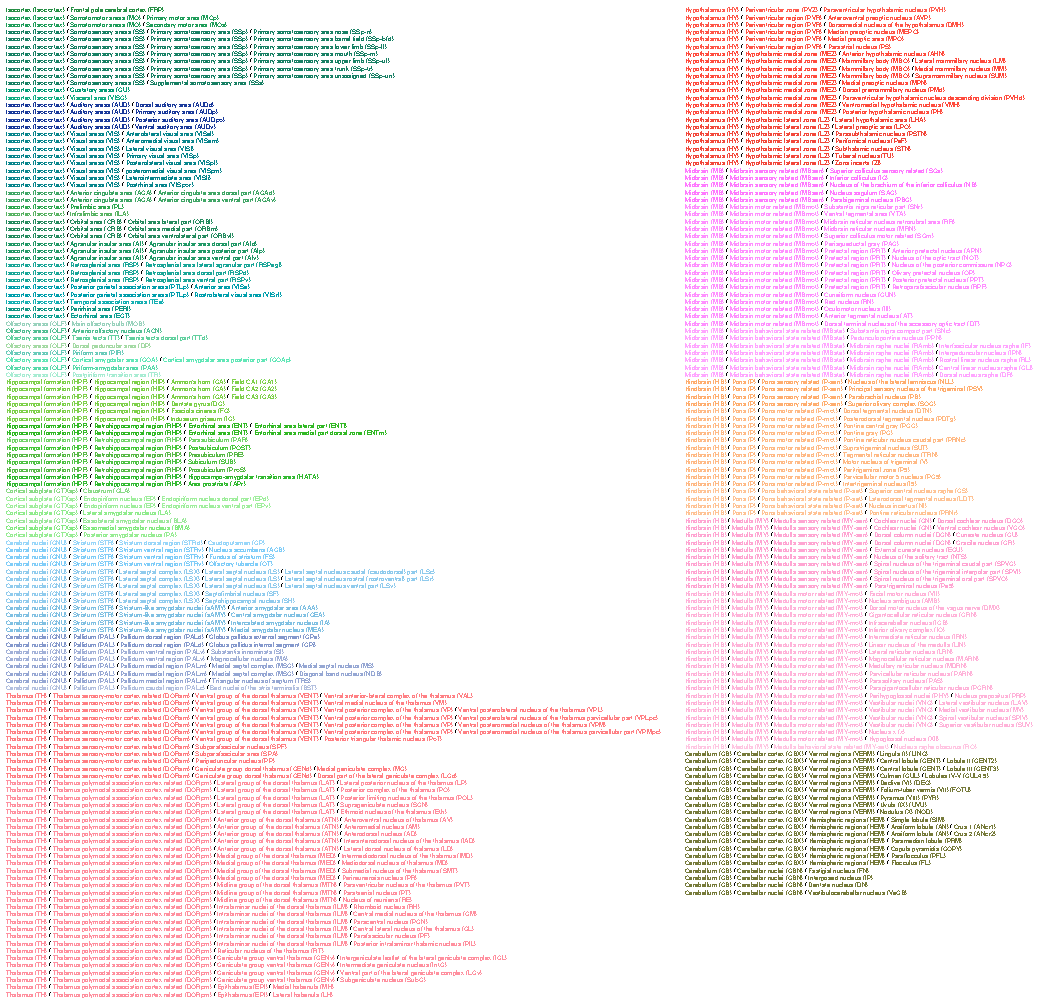
\includegraphics[width=0.85\linewidth]{figures/structure_tree.pdf}
\caption{\textbf{Anatomical hierarchy for all used regions}
For each of the used regions, at "Beryl" hierarchical level, the parent structures are shown with full names and acronyms, up to "Cosmos" hierarchical level. Find the full anatomical hierarchy tree at \href{https://atlas.brain-map.org/atlas}{the Allen adult mouse brain atlas}.
\label{fig:recorded_regions_tree}
}
\end{fullwidth}
\end{figure}
